\chapter{Conclusion and Future Directions}
\label{chpt:conclusion}

This dissertation has presented three distinct projects that propose or highlight innovations in likelihood based inference of state space models, an important tool for time series analysis.
In Chapter~\ref{chpt:arima}, I demonstrate how even simple linear Gaussian state space models can cause challenges for likelihood based inference.
Specifically, existing algorithms for fitting ARIMA models nominally maximize model likelihoods, but fail to do so for a surprisingly large number of instances.
The proposed algorithm helps address these optimization shortcomings.
Given the importance of ARIMA models to modern science, the proposed algorithm may constitute a significant advancement of statistical practice.

In Chapter~\ref{chpt:haiti}, I demonstrate how state space models can be used to make inference on dynamic systems and consequently inform policy decisions.
An important feature of state space models is they allow researchers to include mechanisms that reflect our current understanding of how dynamic systems of interest evolve over time.
This feature enables estimation of the impacts of potential system interventions, such as the introduction of masking or vaccination policies.
In this project, I argue that model based recommendations should be strongly supported by data that were generated from the system of interest.
Currently accepted standards for model based recommendations unfortunately often do not satisfy this criteria, and this project highlights this deficiency while proposing a reproducible workflow to aid in this task.

Chapter~\ref{chpt:mpif} proposes a novel algorithm for performing maximum likelihood estimation for high-dimensional PanelPOMP models.
Existing procedures for this task exist, though the lack of applications in existing literature suggests that current statistical methodologies have practical limitations.
The utility of the proposed algorithm is demonstrated on a series of simulation studies, and is found to be superior to existing alternatives for maximum likelihood.
Theoretical support for the new algorithm is provided via an analysis of iterating a Bayesian inference update followed by a marginalization procedure.

Recent advances in machine learning and artificial intelligence (AI) have significantly enhanced researchers' ability to extract information from complex data sets.
Consequently, much of the recent enthusiasm and effort in statistics and computational science over the last decade has been dedicated to expanding the limits, capabilities, and applications of these fields.
While the excitement surrounding machine learning and AI is well-justified, state-space models (SSMs) also play a crucial role in advancing scientific understanding \citep{baker18,hogg24}.
For example, SSMs offer greater interpretability compared to machine learning algorithms, making them valuable for inferring features of dynamic systems.
Moreover, by incorporating real-world mechanisms into their formulations, SSMs have the potential to improve predictions and provide more reliable estimates of the impacts of system interventions.
This latter task is particularly challenging for machine learning algorithms, which depend on existing data, as hypothetical interventions represent counter factual scenarios not present in the data.

Advances in SSM methodology may also play a crucial role in advancing machine learning and AI.
As summarized by \citet{lin24}, the large language models that have been the driving force behind the success of generative AI are based on non-mechanistic SSMs treated as input-output mapping modules.
As a result, innovations in likelihood based inference for SSMs could lead to novel techniques for designing and calibrating AI models in ways that are not yet fully understood.
Likelihood based inference for state space models is a large and challenging topic, and this thesis only presents a few innovations related to this problem.
Below, I outline several future projects that build on the work presented in this dissertation.

\subsection*{Estimation for Nested PanelPOMP models}

One of the promising applications of PanelPOMP methodology and software is to analyze designed experiments of dynamic systems.
Currently, existing approaches can work well for systems where each replicate of the experiment is treated as a distinct POMP model and distinct features (or parameters) are unique to the replicates themselves or are otherwise shared across all replicates.
Using the language of Chapter~\ref{chpt:mpif}, this means that there are a single set of shared parameters for all experimental replicates, and each replicate has unit-specific parameters. 
In more complicated designs, however, there may additionally be features shared between replicates of the same experimental treatment, resulting in shared parameters at two distinct levels.
More complex designs are also of interest, and methodology enabling inference in these circumstances should be developed.
Notably, methodology that enables multiply nested parameter estimation can be useful in observational studies with similarly structured data. 

\begin{figure}[h!]
    \centering
    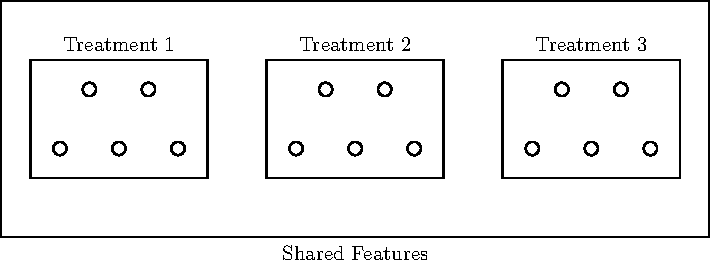
\includegraphics[width=0.7\linewidth]{chapters/conclusion/nestedDesign.pdf}
    \caption[A diagram of a controlled experiment with replications.]{A diagram of a controlled experiment with replications. Each circle represents a unique replicate with its own distinct features (parameters). The rectangular boxes represent different treatments, each containing shared features for their respective replications. The entire experiment is encased in a larger rectangle indicating features common across all treatments.}
    \label{fig:controlled_experiment}
\end{figure}

The theoretical analysis of the PIF algorithm presented in Chapter~\ref{chpt:mpif} can readily be extended to include this extra layer of parameter nesting, though existing software cannot immediately be used to handle this general scenario.

\subsection*{Parameter estimation using automatic differentiation}

Recent methodological work on automatic differentiation for particle filters has shown potential for speeding up inference for POMP models \citep{tan24}.
The MPIF algorithm presented in Chapter~\ref{chpt:mpif} can be immediately combined with this promising methodology in the panel setting, as the method of \citet{tan24} requires a warm restart in order to successfully converge to the MLE.

Additionally, the combination of MPIF and automatic differentiation may facilitate the use of shallow neural networks to be used in conjunction with mechanistic models.
As an example, consider a continuous time compartmental model outlined in Appendix~\ref{subsec:smcs}.
Transition rates between compartments are generally expressed as functions of latent and exogenous variables, denoted $f(\bm{X}(t), \bm{Z}(t))$.
Rather than predetermining the function $f$, automatic differentiation software may enable treating $f$ as a flexible function that needs to be estimated.
A similar idea has been explored previously \citep{noordijk24,dandekar20}, though only in the context of deterministic ODE models, or SDE models with non-mechanistic latent dynamics \citep{lin24}.
In the later approach, a neural network is used to approximate an unknown function that describes the latent process. 
This has the advantage of allowing flexible description of latent states, but it loses the benefits of being mechanistic.
Automatic differentiation for particle filters instead may allow for retaining the general mechanistic framework of a SSM, while permitting extra flexibility for model components where a mechanistic representation is not readily available \citep{dandekar20}. 

\subsection*{Applications in Ecology, Agriculture, and Epidemiology}

The MPIF algorithm presented in Chapter~\ref{chpt:mpif} results in an improved capacity to calibrate PanelPOMP models to data via maximum likelihood.
Given the prevalence of panel data and applications of POMP models to univariate time series, this innovation may lead to a number of collaborative research projects in epidemiology.
Iterated filtering has been a poplar approach for modeling infectious disease outbreaks at a single measurement location using nonlinear, overdispersed stochastic models \citep[e.g.,][]{stocks20}. 
The MPIF algorithm facilitates fitting similar models to outbreaks measured at various distinct locations, which can be particularly useful at the onset of disease outbreaks, when there is limited amounts of data available at a single measurement location.

In addition to novel applications in epidemiology, there are several areas of research where I feel that PanelPOMP methodology can lead to novel scientific insights.
Two application areas I feel are particularly promising are fisheries and agriculture.
Fisheries have a rich history of using state space models, though typically inference is performed using Lapacian approximations of the likelihood \citep[e.g.,][]{auger17}.
In addition to comparing whether this approach is a more reliable approximation that those built on sequential Monte Carlo methodologies, studying infectious diseases prevalent in native river and lake species may be uniquely well suited for PanelPOMP methodology: population dynamics in each river or lake are independent from other locations, yet share many similar features that should be estimated simultaneously.
Alternatively, the MPIF methodology may be used to model the nonlinear stochastic dynamics that arise from distinct fish populations competing for the same finite resources \citep{rosenthal22}.
Fish populations exhibit many of the same obstacles for inference that were outlined by \citet{bjornstad01}, and iterated filtering based algorithms have been successfully used to the same challenges in infectious disease outbreaks.

Livestock populations also exhibit nonlinear, stochastic features of biological systems, and may be well suited for applying PanelPOMP methodology.
Recently published research on livestock management \citep{skolstrup22} used linear Gaussian state space models to estimate the effects of interventions at dairy farms, and methodologies enabling nonlinear models may be a natural next step.
The MPIF algorithm may be used to fit nonlinear SSMs for large collections independent time series data, and could be useful for controlling infectious disease outbreaks such as recent avian flu outbreaks \citep{pinotti24}.

\subsection*{Likelihood based inference for ARIMA models}

In Chapter~\ref{chpt:arima}, a new algorithm was presented for performing maximum likelihood estimation for the parameters of an ARIMA model.
This project resulted in the development of an R package called \code{arima2}, which has already been downloaded more than the majority of R packages available on the Comprehensive R Archive Network (CRAN).
Given the importance of ARIMA models to modern science, additional efforts to improve both the algorithm and improve access to the algorithm are warranted.
For instance, a Python package that implements the algorithm should be built in order to provide access to help practitioners that prefer the Python language for data analysis.
Additional modifications to the algorithm may could include stratified sampling of parameter coefficients.
Alternatively, theoretical developments that provide bounds on the number of local optima could be explored. 
